%pdflatex
\documentclass[A4]{article}

\usepackage{tikz,tikzpagenodes,a4wide,lipsum}
\usetikzlibrary{calc}

\title{Title Page}

\begin{document}

\begin{titlepage}

\begin{tikzpicture}[overlay,remember picture]
\draw [line width=1.0pt,rounded corners=10pt,]
    ($ (current page.north west) + (2.5cm,-3.5cm) $)
    rectangle
    ($ (current page.south east) + (-3.5cm,2.5cm) $);       
\end{tikzpicture}

\begin{center}
        \vspace*{1cm}

        \huge
        \textbf{Sample title page with border}

        \vspace{2.0cm}
        \LARGE
        \textbf{First name, Family name}

        \vfill

        \Large
         Date: Today
\end{center}
\end{titlepage}

\clearpage

\begin{minipage}{.5\textwidth}
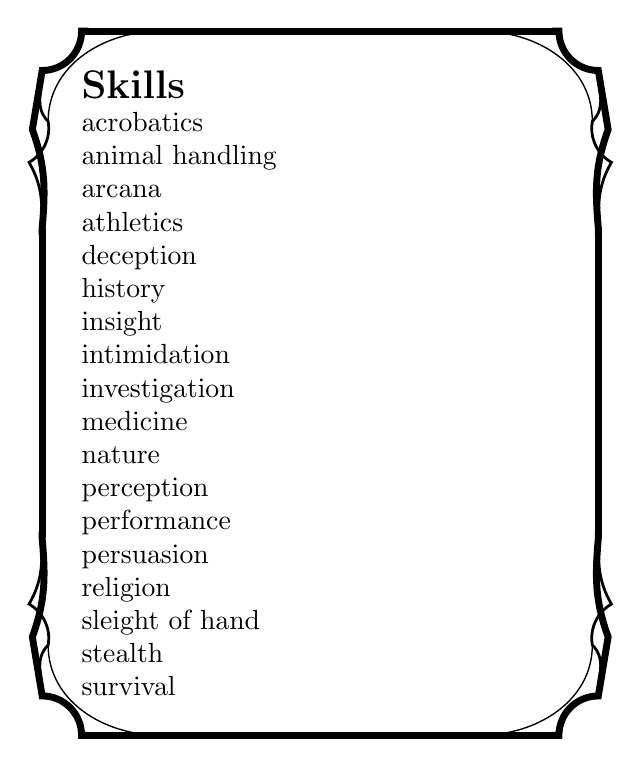
\begin{tikzpicture}
\begin{scope}
\node[inner sep=0pt,outer sep=0pt,text width=0.5\textwidth](t){%
{\Large\bfseries Skills}\par%
  acrobatics \\
  animal handling \\
  arcana \\
  athletics\\
  deception\\
  history\\
  insight\\
  intimidation\\
  investigation\\
  medicine\\
  nature\\
  perception\\
  performance\\
  persuasion\\
  religion\\
  sleight of hand\\
  stealth\\
  survival
};

\def\dnddrawsize{5mm}

\def\dndhoroffset{5mm}
\def\dndveroffset{25mm}

\def\dndfatline{2.5pt}
\def\dndmedline{1.0pt}
\def\dndthinline{0.5pt}

\coordinate (O) at ($(t.north west) + (-2*\dnddrawsize, 2*\dnddrawsize)$);
\coordinate (A) at ($(t.north east) + ( 2*\dnddrawsize, 2*\dnddrawsize)$);
\coordinate (B) at ($(t.south east) + ( 2*\dnddrawsize,-2*\dnddrawsize)$);
\coordinate (C) at ($(t.south west) + (-2*\dnddrawsize,-2*\dnddrawsize)$);

\coordinate (o) at ($(t.north west) + (-\dnddrawsize, \dnddrawsize)$);
\coordinate (a) at ($(t.north east) + ( \dnddrawsize, \dnddrawsize)$);
\coordinate (b) at ($(t.south east) + ( \dnddrawsize,-\dnddrawsize)$);
\coordinate (c) at ($(t.south west) + (-\dnddrawsize,-\dnddrawsize)$);

%\path[clip] ($(O) + (-.5pt,.5pt)$)
%	rectangle
%	($(B) + (.5pt,-.5pt)$);

% lines
\draw[line width=\dndfatline, shorten <= \dndhoroffset, shorten >= \dndhoroffset] (o) -- (a);
\draw[line width=\dndfatline, shorten <= \dndveroffset, shorten >= \dndveroffset] (a) -- (b);
\draw[line width=\dndfatline, shorten <= \dndhoroffset, shorten >= \dndhoroffset] (b) -- (c);
\draw[line width=\dndfatline, shorten <= \dndveroffset, shorten >= \dndveroffset] (c) -- (o);

% top left corner
\draw[line width=\dndfatline]
	($ (o) + (\dndhoroffset, 0) + (\dndfatline, 0) $)
	-- ($ (o) + (\dndhoroffset, 0) $)
	arc (0:-90:\dndhoroffset)
	-- ($ (o) + (-\dndhoroffset/4,-\dndveroffset/2)$)
	to[in=85,out=290] ($ (o) + (0,-\dndveroffset) $)
	-- ($ (o) + (0,-\dndveroffset) + (0, -\dndfatline) $)
;
\draw[line width=\dndmedline]
	($ (o) + (0,-\dndveroffset) $)
	to[in=300,out=90] ($ (o) + (-\dndhoroffset/3,-2*\dndveroffset/3) $)
	arc (300:370:\dndhoroffset)
	coordinate (o2)
	to[in=270,out=135] ($ (o) + (0,-\dndhoroffset) $)
;
\draw[line width=\dndthinline]
	(o2)
	to[in=180,out=90]
	($ (o) + (3*\dndhoroffset,0) $)
;

% top right corner
\draw[line width=\dndfatline]
	($ (a) + (-\dndhoroffset, 0) + (-\dndfatline, 0) $)
	-- ($ (a) + (-\dndhoroffset, 0) $)
	arc (180:270:\dndhoroffset)
	-- ($ (a) + (\dndhoroffset/4,-\dndveroffset/2)$)
	to[in=95,out=250] ($ (a) + (0,-\dndveroffset) $)
	-- ($ (a) + (0,-\dndveroffset) + (0, -\dndfatline) $)
;
\draw[line width=\dndmedline]
	($ (a) + (0,-\dndveroffset) $)
	to[in=240,out=90] ($ (a) + (\dndhoroffset/3,-2*\dndveroffset/3) $)
	arc (240:170:\dndhoroffset)
	coordinate (a2)
	to[in=270,out=45] ($ (a) + (0,-\dndhoroffset) $)
;
\draw[line width=\dndthinline]
	(a2)
	to[in=0,out=90]
	($ (a) + (-3*\dndhoroffset,0) $)
;

% bottom right corner
\draw[line width=\dndfatline]
	($ (b) + (-\dndhoroffset, 0) + (-\dndfatline, 0) $)
	-- ($ (b) + (-\dndhoroffset, 0) $)
	arc (180:90:\dndhoroffset)
	-- ($ (b) + (\dndhoroffset/4,\dndveroffset/2)$)
	to[in=265,out=110] ($ (b) + (0,\dndveroffset) $)
	-- ($ (b) + (0,\dndveroffset) + (0, \dndfatline) $)
;
\draw[line width=\dndmedline]
	($ (b) + (0,\dndveroffset) $)
	to[in=120,out=270] ($ (b) + (\dndhoroffset/3,2*\dndveroffset/3) $)
	arc (120:190:\dndhoroffset)
	coordinate (b2)
	to[in=90,out=-45] ($ (b) + (0,\dndhoroffset) $)
;
\draw[line width=\dndthinline]
	(b2)
	to[in=0,out=-90]
	($ (b) + (-3*\dndhoroffset,0) $)
;

% bottom left corner
\draw[line width=\dndfatline]
	($ (c) + (\dndhoroffset, 0) + (\dndfatline, 0) $)
	-- ($ (c) + (\dndhoroffset, 0) $)
	arc (0:90:\dndhoroffset)
	-- ($ (c) + (-\dndhoroffset/4,\dndveroffset/2)$)
	to[in=275,out=70] ($ (c) + (0,\dndveroffset) $)
	-- ($ (c) + (0,\dndveroffset) + (0, \dndfatline) $)
;
\draw[line width=\dndmedline]
	($ (c) + (0,\dndveroffset) $)
	to[in=60,out=270] ($ (c) + (-\dndhoroffset/3,2*\dndveroffset/3) $)
	arc (60:-10:\dndhoroffset)
	coordinate (c2)
	to[in=90,out=-135] ($ (c) + (0,\dndhoroffset) $)
;
\draw[line width=\dndthinline]
	(c2)
	to[in=180,out=-90]
	($ (c) + (3*\dndhoroffset,0) $)
;
	
\end{scope}
\end{tikzpicture}
\end{minipage}

%\begin{minipage}{.5\textwidth}
%\begin{tikzpicture}[overlay][remember picture]
%	\draw [line width=1.0pt,rounded corners=10pt]
%		($ (current bounding box.north west) $)
%		rectangle
%		($ (current bounding box.north west) + (5cm, -5cm)$);
%\end{tikzpicture}
%\end{minipage}

%\begin{minipage}[b][10cm]{.5\textwidth}
%\begin{tikzpicture}[overlay,remember picture]
%\draw [line width=1.0pt,rounded corners=10pt,]
%    ($ (current bounding box.north west) + (5cm, -5cm) $)
%    rectangle
%    ($ (current bounding box.north east) - (5cm, -5cm)$);
%\end{tikzpicture}
%foo
%\\
%
%bar
%\end{minipage}

\end{document}
